\chapter{Eksperymenty i wydajność}

\section{Odnajdywanie regionów}

Ponieważ wynik algorytmu jest taki sam niezależnie od implementacji, szybkość
wykonania jest jedynym czynnikiem charakteryzującym go. Testy zostały
przeprowadzone na zwykłym komputerze domowym o parametrach: pamięć 3.9 GiB,
procesor: Intel Core 2 3.16GHz (wykorzystywany jest tylko jeden rdzeń) w
przeglądarce Chrome 10.0 (silnik javascript: V8 3.0.12.30). Każdy pomiar został
powtórzony wiele razy, najkorzystniejsze wyniki znajdują się na wykresie \ref{mser}.

\begin{figure}[h!] \centering 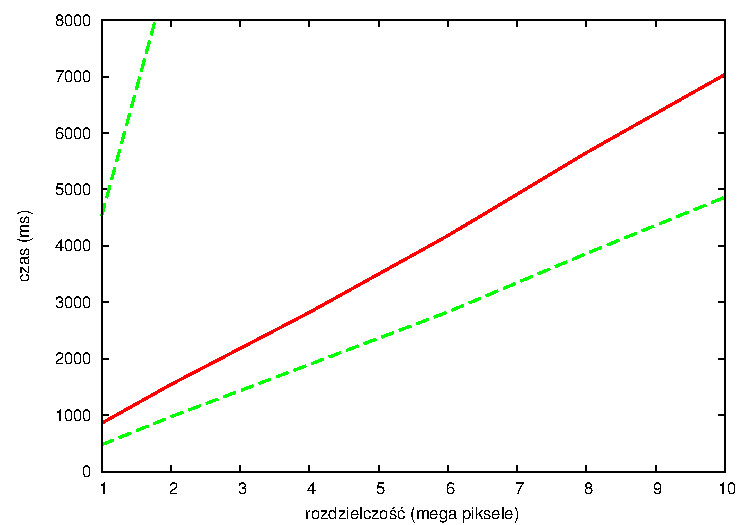
\includegraphics{images/mser.pdf} \caption{Czas
  wykonania pojedynczego przejścia algorytmu MSER+ (od koloru czarnego do
  białego). Dolna linia przerywana powstała po przetworzeniu obrazu o
  jednolitym kolorze (trywialny przypadek), linią ciągłą standardowe zdjęcie z
  aparatu. Obraz zawierający losowe piksele (złośliwy przypadek; wymaga
  utworzenia większego stosu w pamięci) reprezentuje górna linia przerywana.
  Użyte parametry: rozmiar regionu od 50 do 500 pikseli, delta równa 10.}
  \label{mser} \end{figure}

Dla porównania, autorzy \cite{Nister_Stewenius_2008} uzyskali wydajność bliską
5 megapikseli na sekundę. Inne, wcześniejsze implementacje są do dwóch razy
wolniejsze.

\begin{figure}[h!] \centering 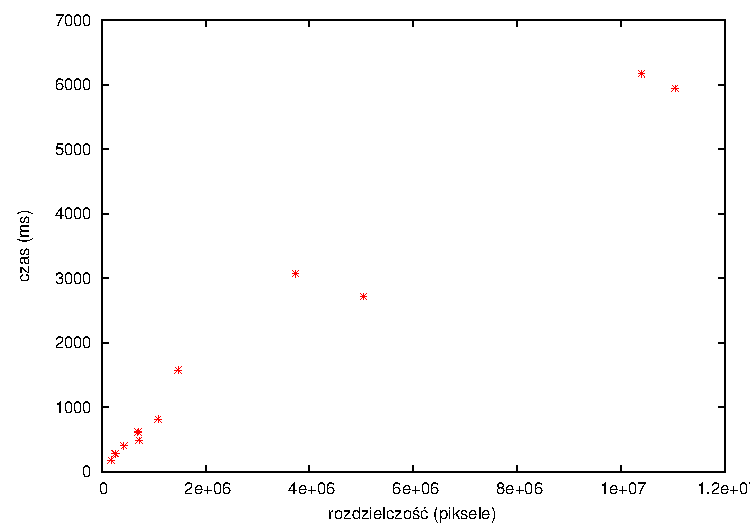
\includegraphics{images/random.pdf}
\caption{Czas wykonania algorytmu MSER+ dla losowo wybranych obrazów w
zależności od rozdzielczości. Czas jest liniowo zależny od rozdzielczości nawet
dla bardzo dużych zdjęć (powyżej 10 megapikseli).} \end{figure}

Ostatni pomiar \ref{delta} ma na celu sprawdzenie czy zmiana parametru $\Delta$
(minimalna różnica jasności między stabilnym regionem a otoczeniem) ma wpływ na
wydajność. Okazuje się, że liczba regionów może tylko w minimalnym stopniu
wpłynąć na czas ich znalezienia.

\begin{figure} \centering
  \subfloat[liczba regionów]{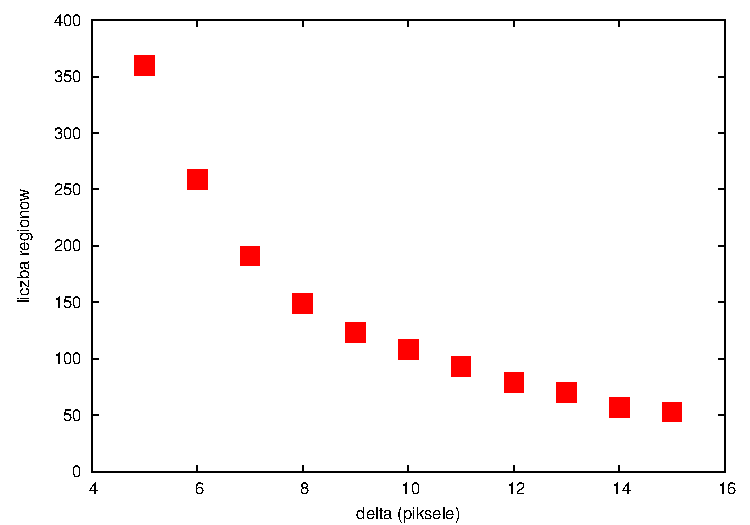
\includegraphics[width=0.5\textwidth]{images/mser_d1.pdf}}
  \subfloat[czas znalezienia]{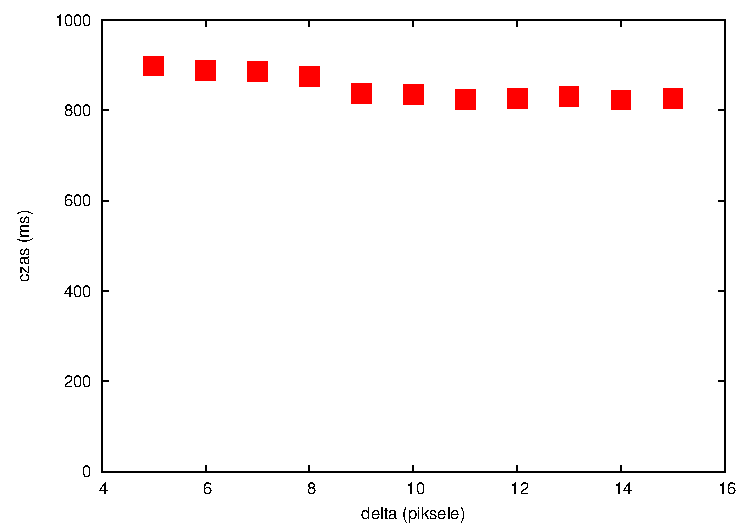
\includegraphics[width=0.5\textwidth]{images/mser_d2.pdf}}
  \caption{Po prawej wpływ parametru $\Delta$ na liczbę znajdywanych obszarów.
  Po lewej wpływ parametru $\Delta$ na czas wykonania algorytmu.} \label{delta}
\end{figure}

%\section{Tymczasowe korespondencje}

%\todo{znalezione korespondencje na znanym zbiorze}

\section{Budowa macierzy fundamentalnej}

Po pierwszych próbnych ewaluacjach algorytmu \cite{eight_point} widać, że
wartości wszystkich obliczanych macierzy fundamentalnych są do siebie bardzo
podobne i zbliżone do następujących wartości: \begin{equation} F =
  \begin{pmatrix} 10^{-4} & 10^{-4} & 10^{-2} \\ 10^{-4} & 10^{-4} & 10^{-2} \\
    10^{-2} & 10^{-2} & 1 \end{pmatrix}.  \end{equation} Ułomność tą zauważył
    również R. Hartley w \cite{defence_8pt}. Wynika ona z tego, że wartości
    współrzędnych, podczas mnożenia macierzy, są redukowane o kilka rzędów
    wielkości (rozważany był przypadek obrazu o standardowej rozdzielczości 200
    pikseli). Rozwiązaniem tego problemu jest normalizacja punktów w taki
    sposób, aby średnia odległość od środka układu współrzędnych była równa
    $\sqrt{2}$ (co odpowiada średniemu punktowi $(1,1,1)^T$). W tym celu
    wskazane jest również przesunięcie początku układu współrzędnych na środek
    ciężkości wszystkich punktów. W ten sposób mamy pewność, że w wyniku
    normalizacji, żadna wartość nie będzie dyskryminowana, a końcowy wynik
    będzie dokładny.

Algorytm \cite{eight_point} z definicji wymaga tylko 8 par punktów, ale
eksperymenty pokazują, że dopiero korzystanie z 20 lub więcej par da pewny
wynik o dostatecznie małym błędzie. 

%\todo{pomiar błędu}
%\todo{błąd w zależności od liczby par}

Rozłożenie punktów na obrazie ma wpływ na dokładność wyniku. Korzystne jest jak
największe ich rozproszenie. Jeżeli wszystkie punkty znajdą się w niedalekiej
od siebie odległości, błędy mogą ulec kulminacji.

Znalezione linie epipolarne mogą się nie przeciąć w jednym punkcie (epipolu).
Jest to sygnał, że jedna (lub więcej) z nich jest błędna i należy ją odrzucić.
Z przeprowadzonych eksperymentów wynika, że uzasadnione jest założenie
położenia epipola po przecięciu się trzech linii w tym samym punkcie. Samo
położenie tego punktu nie jest istotne z punktu widzenia matematycznego, ale
stanowi ono pewną metodę weryfikacji i upewnienia się o poprawności uzyskanego
wyniku. Do dalszych obliczeń związanych z geometrią epipolarną wystarczy tylko
jedna poprawna macierz fundamentalna.

%\section{Dopasowanie linii do zbioru punktów}

\section{Podsumowanie}

Wyszukiwanie stabilnych regionów obrazu to najbardziej czasochłonny algorytm w
procesie obliczania geometrii epipolarnej sceny. W chwili obecnej moja
implementacja nie jest w stanie reagować na zmiany parametrów ani obrazu w
czasie rzeczywistym (tj. więcej niż 15 razy na sekundę). Jak pokazują inne
implementacje jest to jednak jak najbardziej możliwe, ale wymaga dodatkowej
pracy.  W dalszej perspektywie daje to nadzieję, na łatwy sposób budowy
np. użytecznych aplikacji internetowych rozumiejących obrazy.
